\documentclass{article}
\usepackage{v-test-paper}
\renewcommand{\ans}{\quad}
\def\ansint#1{\quad}
\title{Test-Paper\\(Physics-JEE)}

\begin{document}
\maketitle

\jeeSectionA
\begin{enumerate}
\item If $f_1$, $f_2$ and $f_3$ are the fundamental frequencies of three segments into which a string is divided, then the original fundamental frequency($f_0$) of the whole string is
	\begin{tasks}(2)
		\task $f_0 = f_1 + f_2 + f_3$
		\task $\dfrac{1}{f_0} = \dfrac{1}{f_1} + \dfrac{1}{f_2} + \dfrac{1}{f_3}$\ans
		\task $\dfrac{1}{\sqrt{f_0}} = \dfrac{1}{\sqrt{f_1}} + \dfrac{1}{\sqrt{f_2}} + \dfrac{1}{\sqrt{f_3}}$
		\task None of these
	\end{tasks}



\item A travelling wave is described by the equation\[ y(x, t) = 0.05\sin\left(8x-4t\right)\m\] The velocity of the wave is:
	\begin{tasks}(2)
		\task $2\mps$
		\task $4\mps$
		\task $8\mps$
		\task $0.5\mps$\ans
	\end{tasks}

\item In the wave equation \[ y=0.5\sin\dfrac{2\pi}{\lambda}\left(400t-x\right) \m\] the velocity of the wave will be:
	\begin{tasks}(2)
		\task $200\mps$
		\task $400\mps$\ans
		\task $200\sqrt{2}\mps$
		\task $400\sqrt{2}\mps$
	\end{tasks}

\item A transverse wave is represented by $y=2\sin\left(\omega t -k x\right) \cm$. The value of wavelength (in $\cm$) for which the wave velocity becomes equal to the maximum particle velocity, will be :
	\begin{tasks}(2)
		\task $4\pi$\ans
		\task $2\pi$
		\task $\pi$
		\task $2$
	\end{tasks}

\item Which of the following equations correctly represents a travelling wave having wavelength $\lambda= 4.0 \cm$, frequency $\nu = 100 \Hz$ and travelling in positive x-axis direction? (in all the options $x$ is in $\cm$ and $t$ is in $\s$)
	\begin{tasks}(2)
		\task $y= A\sin\left(0.5\pi x - 100\pi t\right)$
		\task $y= A\sin\left(0.25\pi x - 100\pi t\right)$
		\task $y= A\sin\left(0.5\pi x - 200\pi t\right)$\ans
		\task $y= A\sin\left(0.25\pi x - 200\pi t\right)$
	\end{tasks}

\item A longitudinal wave is represented by $x=10\sin\left(2\pi n t - \dfrac{2\pi}{\lambda}x\right)\cm$. The maximum particle velocity will be four times the wave velocity if the determined value of wavelength is equal to :
	\begin{tasks}(2)
		\task $2\pi$
		\task $5\pi$\ans
		\task $\pi$
		\task $\dfrac{5\pi}{2}$
	\end{tasks}

\item The equations of two waves are given by:
	\begin{align*}
		y_1 &= 5\sin\left(2\pi x - 2\pi v t\right) \cm\\
		y_2 &= 3\sin\left(2\pi x - 2\pi v t + 3\pi\right) \cm
	\end{align*}
	These waves are simultaneously passing through a string. The amplitude of the resulting wave is :
	\begin{tasks}(2)
		\task $2\cm$\ans
		\task $4\cm$
		\task $5.8\cm$
		\task $8\cm$
	\end{tasks}

\item The motion of a mass on a spring, with spring constant $k$ as shown in figure.
	\begin{center}
		\begin{tikzpicture}
			\pic[rotate=-90] (leftwall) at (0, 0){frame=2cm};
			\tzsnake+{5pt}
        [coil,amplitude=5pt,post length=10pt]
        (leftwall-center)(2.5,0)
			\node[block, anchor=west] (block) at(2.5, 0){$m$};
			\tzsnake+[dashed]{5pt}
		[coil,amplitude=5pt,post length=10pt]
		(block.east)(1.5,0)
		\node[block, anchor=west, dashed] (blockdashed) at (4.8,0){$m$};
		\tzline[|<->|]<0, -0.5>(block.south)(blockdashed.south){$x$}[mb]
		\end{tikzpicture}
	\end{center}
	The equation of motion is given by: \[ x(t)=A\sin(\omega t) + B\cos(\omega t) \quad\textit{ with } \omega=\sqrt{\dfrac{k}{m}} \]
	Suppose that at time $t=0$, the position of mass is $x(0)$ and the velocity is $v(0)$, then its displacement can also be represented as $x(t)=C\cos(\omega t - \phi)$, where $C$ and $\phi$ are:
	\begin{tasks}(2)
		\task $C=\sqrt{\dfrac{2v(0)^2}{\omega^2} + x(0)^2}, \quad \phi=\tan^{-1}\left(\dfrac{x(0)\omega}{2v(0)}\right)$
		\task $C=\sqrt{\dfrac{v(0)^2}{\omega^2} + x(0)^2}, \quad \phi=\tan^{-1}\left(\dfrac{x(0)\omega}{v(0)}\right)$
		\task $C=\sqrt{\dfrac{v(0)^2}{\omega^2} + x(0)^2}, \quad \phi=\tan^{-1}\left(\dfrac{v(0)}{x(o)\omega}\right)$\ans
		\task $C=\sqrt{\dfrac{2v(0)^2}{\omega^2} + x(0)^2}, \quad \phi=\tan^{-1}\left(\dfrac{v(0)}{x(0)\omega}\right)$ 
	\end{tasks}

\item A sound wave of frequency $245\Hz$ travels with the speed of $300\mps$ along the positive x-axis. Each point of the wave moves to and from through a total distance of $6\cm$. What will be the mathematical expression of this travelling wave?
	\begin{tasks}(2)
		\task $y(x, t)=0.03\sin\left(5.1 x -0.2\times 10^3 t\right)$
		\task $y(x, t)=0.03\sin\left(5.1 x -1.5\times 10^3 t\right)$\ans
		\task $y(x, t)=0.06\sin\left(5.1 x -1.5\times 10^3 t\right)$
		\task $y(x, t)=0.06\sin\left(0.8 x -0.5\times 10^3 t\right)$
	\end{tasks}

\item Which of the following equations represents a travelling wave?
	\begin{tasks}(2)
		\task $y=Ae^x\cos(\omega t -\theta)$
		\task $y=Ae^{-x^2}(vt+\theta)$
		\task $y=A\sin(15x - 2t)$\ans
		\task $y=A\sin x \cos \omega t$
	\end{tasks}

\item For a transverse wave travelling along a straight line, the distance between two peaks (crests) is $5 \m$, while the distance between one crest and one trough is $1.5 \m$. The possible wavelengths (in m) of the are : 
	\begin{tasks}(2)
		\task $1, 3,  5, \cdots$
		\task $\dfrac{1}{1}, \dfrac{1}{3}, \dfrac{1}{5}, \cdots$ \ans
		\task $1, 2, 3, \cdots$
		\task $\dfrac{1}{2}, \dfrac{1}{4}, \dfrac{1}{6}, \cdots$
	\end{tasks}

\item A uniform thin rope of length $12 \m$ and mass $6 \kg$ hangs vertically from a rigid support and a block of mass $2 \kg$ is attached to its free end. A transverse short wavetrain of wavelength $6 \cm$ is produced at the lower end of the rope. What is the wavelength of the wavetrain (in cm) when it reaches the top of the rope ?
	\begin{tasks}(2)
		\task $6$
		\task $12$\ans
		\task $3$
		\task $9$
	\end{tasks}

\item Two identical strings $X$ and $Z$ made of same material have tension $T_X$ and $T_Z$ in them. If their fundamental frequencies are $450 \Hz$ and $300 \Hz$, respectively, then the ratio $\dfrac{T_X}{T_Z}$ is 
	\begin{tasks}(2)
		\task $2.25$\ans
		\task $0.44$
		\task $1.25$
		\task $1.5$
	\end{tasks}

\item A wire of length $L$ and mass per unit length $6\times 10^{-3}\kg/\m$ is put under tension of $540\N$. Two consecutive frequencies that it resonates are $420\Hz$ and $490\Hz$. Then length $L$ in meters is:
	\begin{tasks}(2)
		\task $5.1\m$
		\task $2.1\m$\ans
		\task $1.1\m$
		\task $8.1\m$
	\end{tasks} 

\item A transverse wave travels on a taut steel wire with a velocity of $v$ when tension in it is $2.06\times 10^4 \N$. When the tension is changed to $T$, the velocity changed to $v/2$. The value of $T$ is close to:
	\begin{tasks}(2)
		\task $5.15\times 10^4 \N$
		\task $2.50\times 10^4 \N$
		\task $1.03\times 10^2 \N$
		\task $5.15\times 10^3 \N$\ans
	\end{tasks}

\item Speed of a transverse wave on a straight wire of mass $6\gm$, length $60\cm$ and area of cross-section $1.0\mm^2$ is $90\mps$. If the Young's modulus of the wire is $16\times 10^{11}\N/\m^2$, the extension of wire over its natural length is:
	\begin{tasks}(2)
		\task $0.03\mm$\ans
		\task $0.04\mm$
		\task $0.02\mm$
		\task $0.01\mm$
	\end{tasks}

\item A progressive wave travelling along the positive x-direction is represented by $y(x, t)=A\sin\left(kx-\omega t + \phi\right)$. Its snapshot at $t=0$ is shown in the figure. For this wave, the phase $\phi$ is:
	\begin{center}
		\begin{tikzpicture}
			\tzaxes(-2*pi, -1.5)(2*pi, 1.5){$x$}{$y$}
			\tzfn{-sin(deg(2*\x))}[-1.5*pi:1.5*pi]
			\tzline[|<->|]<0.25, 0>(0, 0)(0, 1){$A$}[mr]
		\end{tikzpicture}
	\end{center}
	\begin{tasks}(2)
		\task $0$
		\task $\pi$\ans
		\task $\dfrac{\pi}{2}$
		\task $\dfrac{3\pi}{2}$
	\end{tasks}

\item A travelling harmonic wave is represented by the equation $y(x,t) = 10^{-3}\sin (50t + 2x)$, where, $x$ and $y$ are in mater and $t$ is in seconds. Which of the following is a correct statement about the wave ? 
	\begin{tasks}(1)
		\task The wave is travelling in the positive x-direction with a speed of $25\mps$
		\task The wave is travelling in the negative x-direction with a speed of $25\mps$\ans
		\task The wave is travelling in the positive x-direction with a speed of $50\mps$
		\task The wave is travelling in the negative x-direction with a speed of $50\mps$
	\end{tasks}

\item Equation of travelling wave on a stretched string of linear density $5 \gm/\m$ is $y = 0.03 \sin(450 t - 9x)$ where distance and time are measured in SI units. The tension in the string is : 
	\begin{tasks}(2)
		\task $10 \N$
		\task $7.5 \N$
		\task $5 \N$
		\task $12.5 \N$\ans
	\end{tasks}

\item A standing wave is formed by the superposition of two waves travelling in opposite directions. The transverse displacement is given by \[ y(x, t) = 0.5\sin\left(\dfrac{5\pi}{4}x\right)\cos\left(200\pi t\right) \] What is the speed of the travelling wave moving in the positive x-direction?
	\begin{tasks}(2)
		\task $90\mps$
		\task $120\mps$
		\task $50\mps$
		\task $160\mps$\ans
	\end{tasks}
\end{enumerate}

\pagebreak

\jeeSectionB
\begin{enumerate}\addtocounter{enumi}{20}
\item The equation of wave is given by \[ y(x, t) = 10^{-2}\sin\left(320\pi t -\pi x + \dfrac{\pi^2}{2}\right) \] where $x$ and $y$ are in $\m$ and $t$ in $\s$. The speed of the wave is \hrulefill $\km/\h$\ansint{1152}

\item A guitar string of length $90 \cm$ vibrates with a fundamental frequency of $120 \Hz$. The length of the string producing a fundamental frequency of $180 \Hz$ will be \hrulefill $\cm$. \ansint{60}

\item The displacement equations of two interfering waves are given by
	\begin{align*}
		y_1 &= 10\sin\left(\omega t + \dfrac{\pi}{3}\right) \cm\\
		y_2 &= 5\sin\left(\omega t\right) + \sqrt{3}\cos\left(\omega t\right) \cm
	\end{align*}
	respectively. The amplitude of the resultant wave is \hrulefill $\cm$. \ansint{20}

\item The distance between two consecutive points with phase difference of $60^\circ$ in a wave of frequency $500 \Hz$ is $6.0 \m$. The velocity with which wave is travelling is \hrulefill $\km/\s$. \ansint{18}

\item Two travelling waves of equal amplitudes and equal frequencies move in opposite directions along a string. They interfere to produce a stationary wave whose equation is given by \[ y=10\cos\left(\pi x\right)\sin\left(\dfrac{2\pi}{T}t\right) \cm\] The amplitude of the particle at $x=\dfrac{4}{3} \cm$ will be \hrulefill $\cm$. \ansint{5}

\item The percentage increase in the speed of transverse waves produced in a stretched string if the tension is \linebreak increased by $4\%$, will be \hrulefill $\%$. \ansint{2} 

\item Two waves are simultaneously passing through a string and their equations are:
	\begin{align*}
		y_1 &= A_1\sin\left(kx -kvt\right) \\
		y_2 &= A_2\sin\left(kx -kvt + kx_0\right)\\
		A_1 &= 12\mm, A_2=5\mm, x_0=3.5\cm, k=6.28\cm^{-1}
	\end{align*}
	The amplitude of resulting wave will be \hrulefill $\mm$. \ansint{7}

\item Two travelling waves produces a standing wave represented by equation, \[ y(x, t) = 5\cos\left(\dfrac{\pi}{2}x\right)\sin\left(100\pi t\right)\] The node closest to the origin $x>0$ will be at $x=$ \hrulefill . \ansint{1}

\item A steel wire with mass per unit length $7.0\times 10^{-3}\kg/\m$ is under tension of $70\N$. The speed of transverse waves in the wire will be \hrulefill $\mps$. \ansint{100}
	
\item Three one-dimensional mechanical waves in an elastic medium is given as 
	\begin{align*}
		y_1 &= 3A\sin\left(\omega t - kx\right)\\
		y_2 &= A\sin\left(\omega t - kx + \pi\right)\\
		y_3 &= 2A\sin\left(\omega t + kx \right)
	\end{align*}
	are superimposed with each other. The maximum displacement amplitude of the medium particle would \linebreak be \hrulefill $A$. \ansint{4}

\end{enumerate}

\pagebreak

\begin{center}
\texttt{Answer Key}
\begin{multicols}{5}
\begin{enumerate}
\item (b)
\item (a)
\item (b)
\item (c)
\item (d)
\item (a)
\item (b)
\item (c)
\item (a)
\item (a)
\item (b)
\item (a)
\item (b)
\item (a)
\end{enumerate}
\end{multicols}
\end{center}


\end{document}
